\begin{pr}[2.12.15]
Let $A$ be the first player and $B$ be the second player.\\
Suppose that $E=\{u_1v_1, u_2v_2, \dots, u_kv_k\}$.\\
Consider the following strategy for $B$:\\
If $A$ takes $u_i$ in the last step, takes $v_i$.\\
If $A$ takes $v_i$ in the last step, takes $u_i$.\\
$\cuz$ by the definition of $E$, no two edges have an endpoint in common.\\
$\so u_1, v_1, u_2, v_2, \dots, u_k, v_k$ are distinct.\\
$\so$ the above strategy is legal, since $u_iv_i$ are joined by an edge, and $u_i, v_i$ won't be taken before $A$ takes either $u_i, v_i$.\\
This is the winning strategy for $B$ since the game ends either all $u_1, v_1, \dots, u_k, v_k$ are removed (that is, all vertices), after which is $A$'s turn and she does not have a legal move, or $A$ can't remove any $u_i, v_i$.\\
Since there are odd vertices in the graph, such $E$ does not exist.\\
Consider the following strategy:\\
$A$ removes the vertex $v$ in her first step, and then after each $B$'s step:\\
If $B$ takes $u_i$ in the last step, takes $v_i$.\\
If $B$ takes $v_i$ in the last step, takes $u_i$.\\
This strategy is legal, since $u_iv_i$ are joined by an edge, and $u_i, v_i$ won't be taken before $A$ takes either $u_i, v_i$.\\
This is the winning strategy for $A$ since the game ends either all $v, u_1, v_1, \dots, u_7, v_7$ are removed (that is, all vertices), after which is $B$'s turn and he does not have a legal move, or $B$ can't remove any $u_i, v_i$.\\
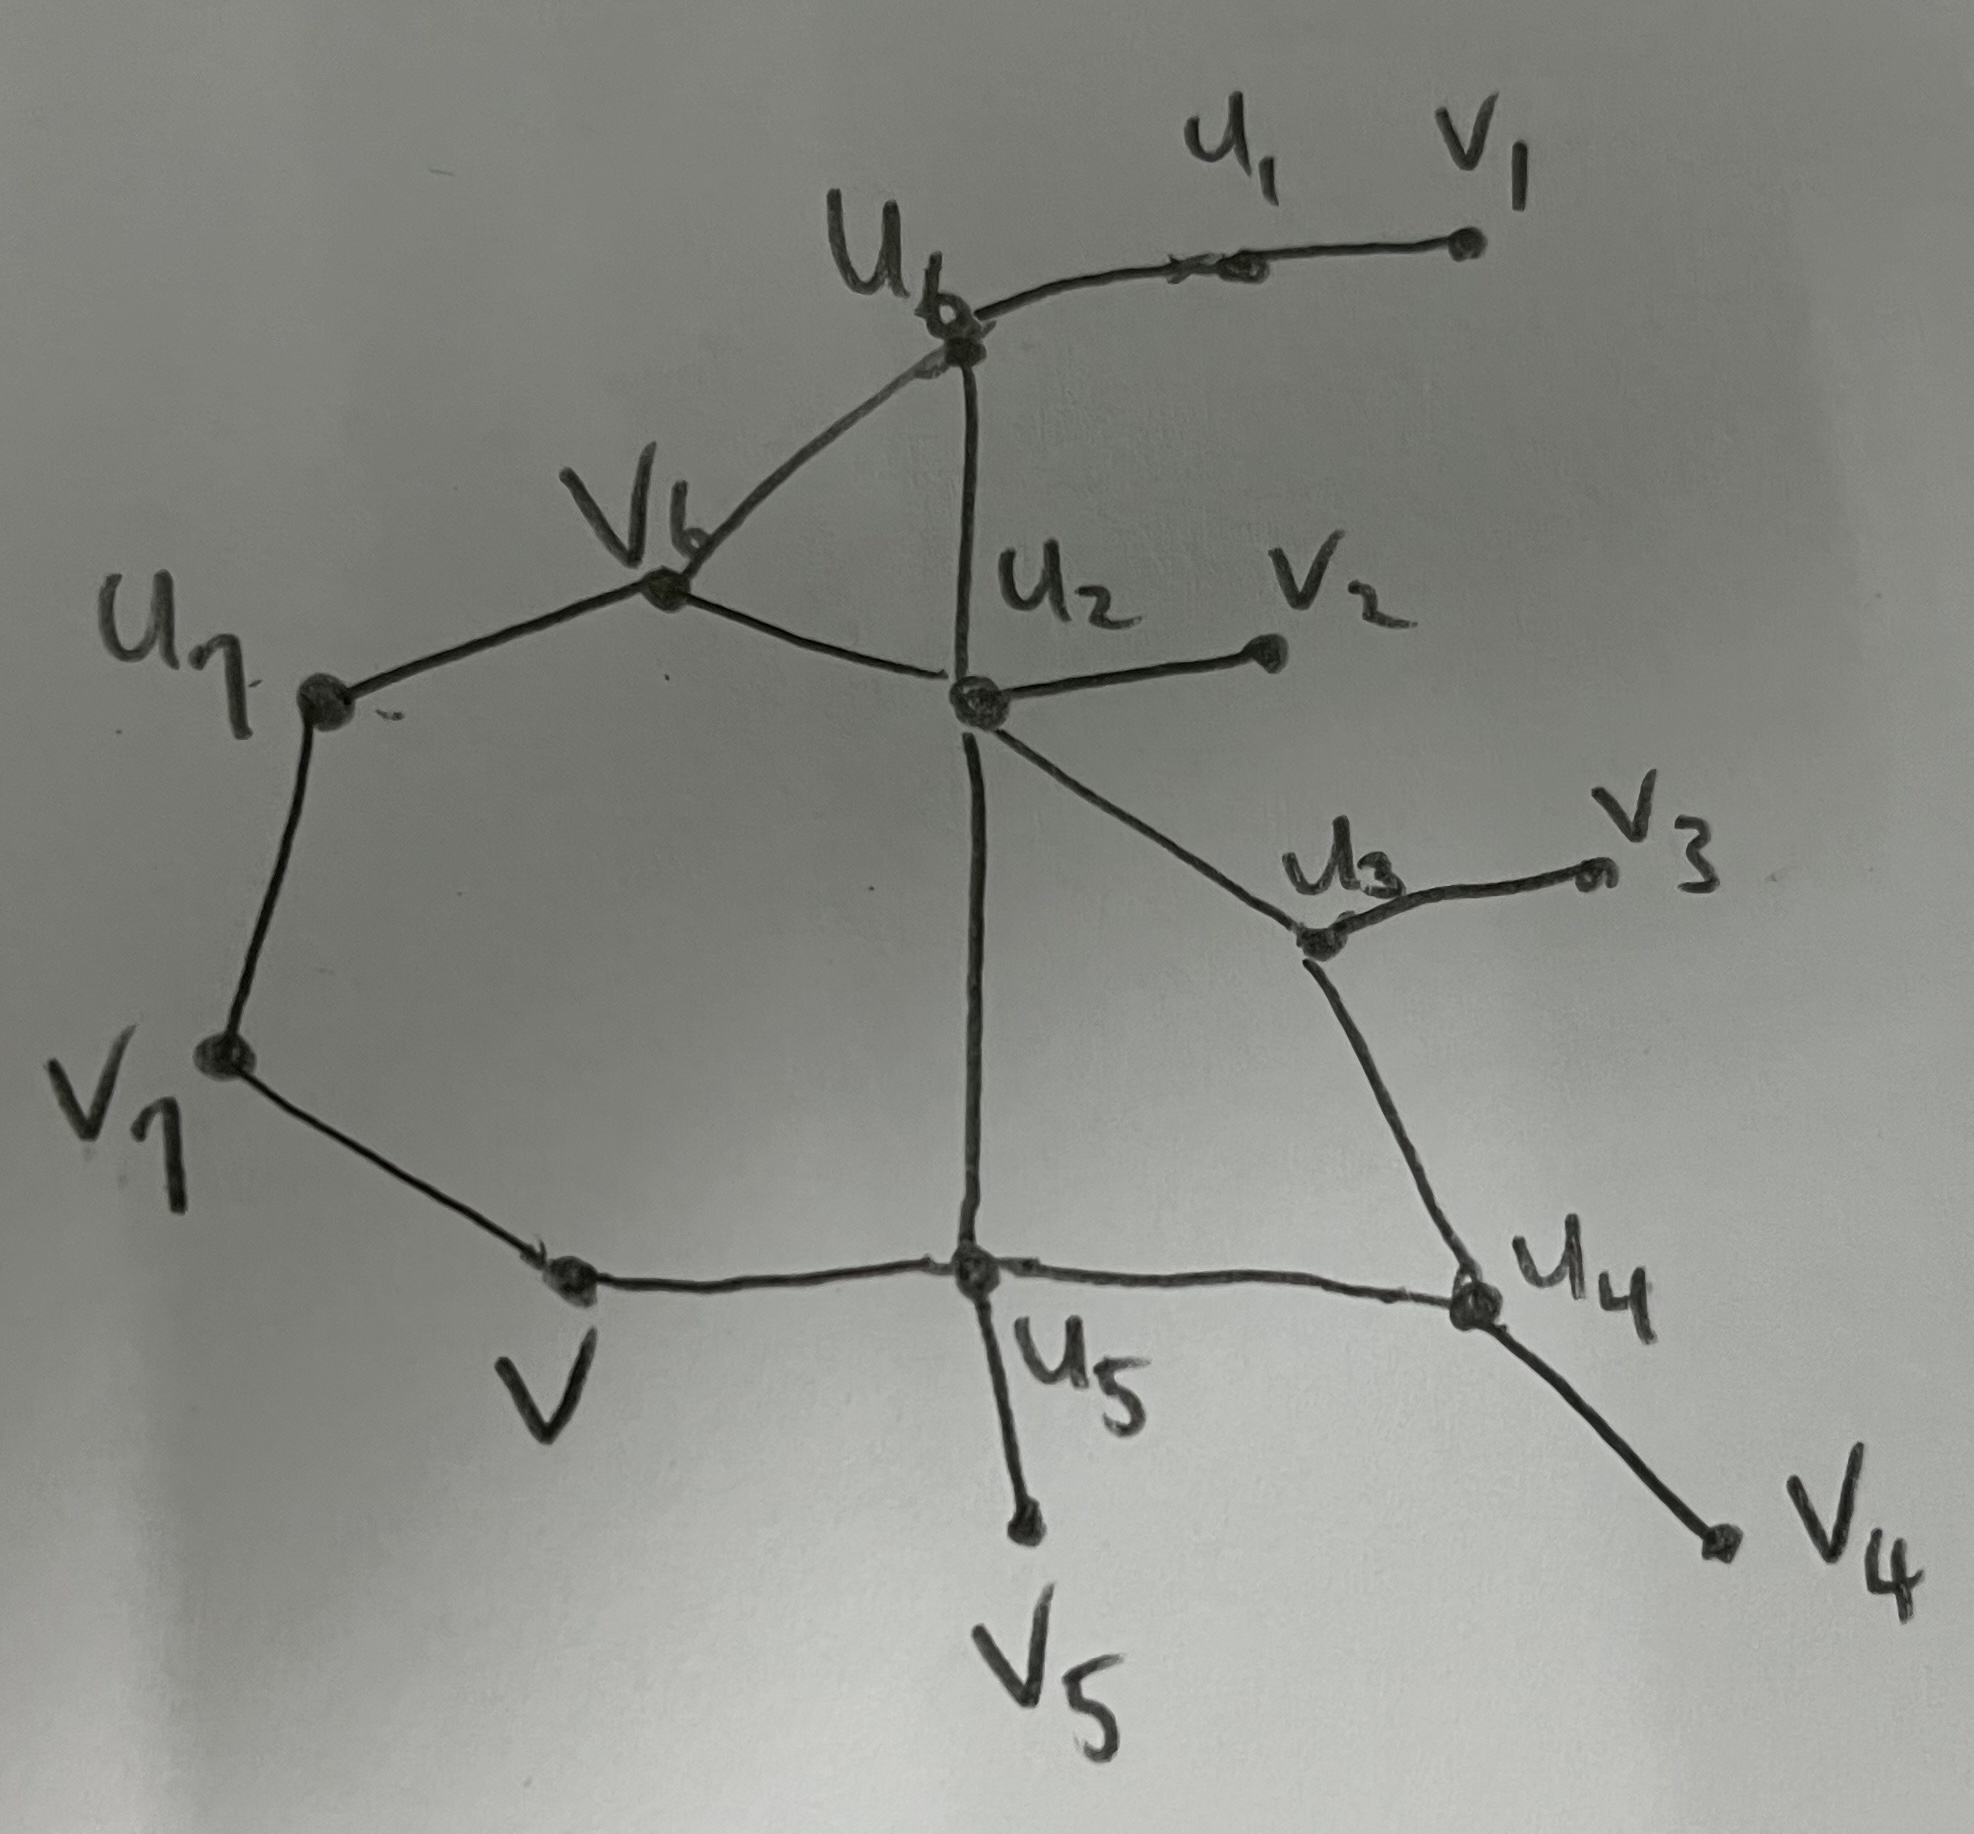
\includegraphics[width=7cm]{p3.JPG}
\end{pr}

\newpage
